\title{(08) Complex Variables}
\author{Ryan Greenup}
\date{Autumn 2019}

\documentclass[class=article, crop=false]{standalone}
\usepackage{./resources/style}

\begin{document}
	\maketitle
	\tableofcontents
	
	
	
\section{Functions of a Complex Variable}
A complex function is a function from a complex plane onto another complex + ane:
\begin{align*}
  A, B \subseteq \mathbb{C} &, \\
  & f: A \rightarrow B
\end{align*}

All the usual definitions of functions still apply, e.g.: 
\\ \

\hfill\begin{minipage}{\dimexpr\textwidth-3cm}
  \begin{itemize}
    \item Functions are rigourously defined using sets 
    \item There is a do main, range, codomain, image etc.
    \item $\dots$
  \end{itemize}
\end{minipage}
\\ \

The \textit{Churchill's} Textbook mentions these conventions however
\begin{enumerate}
  \item Usually the codomain is taken as the set of all complex values.
  \item Most of the results concerning real functions are taken as already established without justification
  \item $x, y, u, v$ denote real variables where as  $z$ and $w$ denote complex variables
    \subitem $z = x +  i y$ 
    \subitem w = u +  i v
    \subitem $f(z) = w \implies f\left( z \right) = u +  iv$
  \item Sometimes there won't be a clear distinction between the values of a function and the function itself, e.g.:
    \begin{align*}
      g\left( z \right) &=  z^2\\
      f\left( g\left( z \right) \right) &=  f\left( z^2 \right)  &\text{Here $z^2$ is shorthand for the function}
    \end{align*}
\end{enumerate}

\newpage
\section{Geometric Interpretation}
Imagine the real function $y = 3$ :
\begin{figure}[!h]
	\centering
	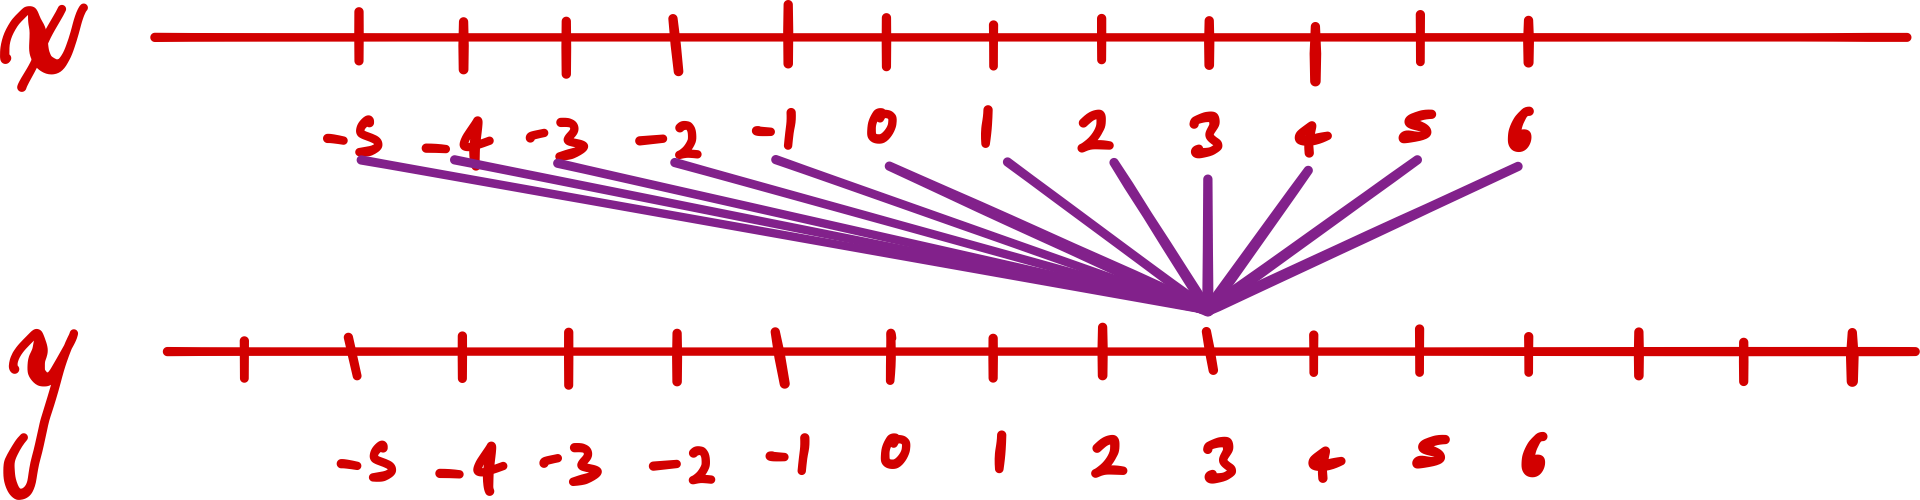
\includegraphics[width=0.7\linewidth]{"./media/ComplexFunctions/PNG image.png"}
	\caption{}
	\label{fig:png-image}
\end{figure}

A similar constant complex function would be $f\left( z \right) =  3 +  4i$:
\begin{figure}[h!]
	\centering
	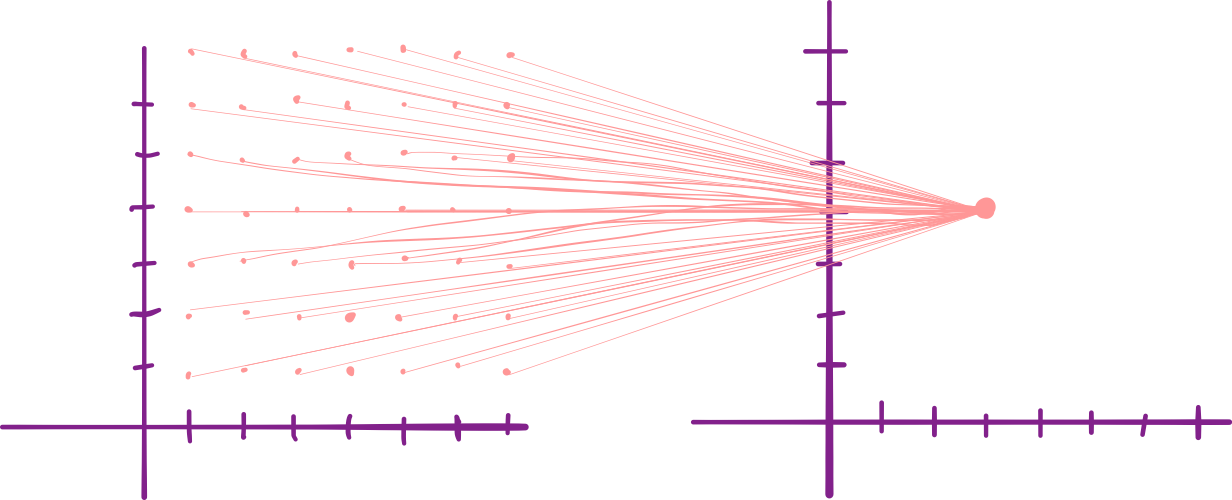
\includegraphics[width=0.7\linewidth]{"./media/ComplexFunctions/PNG image 2.png"}
	\caption{}
	\label{fig:png-image-2}
\end{figure}

It isn't possible to make a graph like it is with simple single variable real functions because that would require four spacial dimensions in order to plot it, this has the dissapointing consequence that geometric interpretations of derivatives as a slope and integrals as area beneath a curve are no longer helpful. \\

It isn't uncommon to use a 3D Cartesian plane to illustrate a function from the reals onto the complex, e.g. imagine $ y =  x^{2}$, if a complex domain is ullustrated as an $x$ /$y$ plane and a perpendicular $z$-axis represents the real codomain, the surface representing the values would always have two roots, even if the're not real, the \textit{Welch Labs} video \textit{Imaginary Numbers are real}\footnote{https://www.youtube.com/watch?v=T647CGsuOVU} is really good for getting a visualisation of this but the general visualisation is:


\begin{figure}[h!]
	\centering
	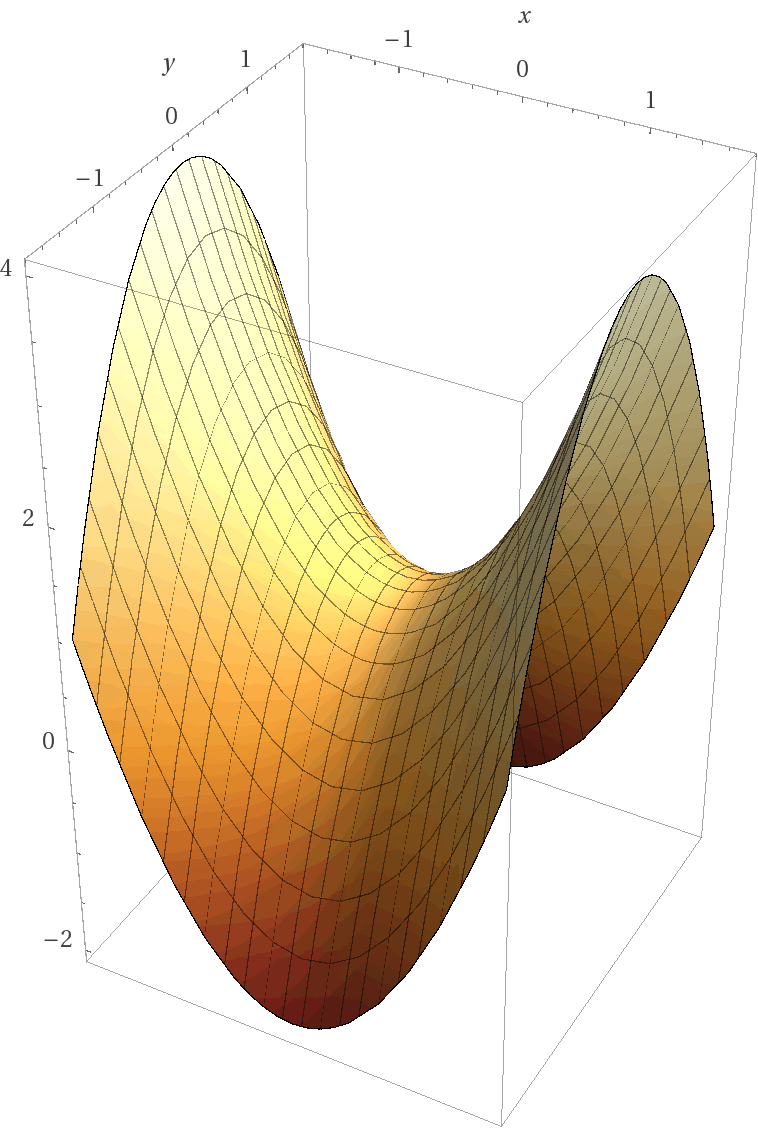
\includegraphics[width=0.2\linewidth]{"./media/ComplexFunctions/PNG image 3.png"}
        \caption{This can be generated in \textit{Wolfram} or something else by using $f(x,y) = \left( x +  i y \right)^2 +  1$}
	\label{fig:png-image-3}
\end{figure}


\section{Complex functions Components}
Complex functions can be illustrated as a pair of two-variable real functions.
Take a function:
\[
  f\left( z \right) =  w
\]
The $w$ variable can be expanded:

\[
  f\left( z \right) =  u +  iv
\]
the $z$ variable can also be expanded:
\[
  f\left( x +  i y  \right) =  u +  iv
\]
Observe that the value $ u$ is in essence a function of the $x$ and $y$ input variables, the same is true also for $v$,  hence, this can be rewritten:

\[
  f\left( x +  i y \right) =  u \left( x,y \right) +  i \times v\left( x,y \right)
  \]

\paragraph{Example}
\begin{align*}
  f\left( z \right) &= z^2 \\
  &= \left( x +  iy  \right)^{2} \\
  &=  x^2 - y^2 +  i \cdot 2xy \\
  &=  \left( x^2 - y^2  \right) +  i \cdot \left( 2xy \right)
  \intertext{So in this case the component functions would be:}
  u\left( x,y \right) &=  \left( x^2 -  y^2 \right) &&\text{and,}\\
  v\left( x,y \right) &=  \left( 2xy \right)
\end{align*}

Essentially a complex-valued function is a pair of two variable real functions.
\subsection{Limits}
if $f$ is defined on all poiints in a \textit{deleted neighbourhood} of $\alpha$ it is written:
\[
  \lim_{z \rightarrow \alpha}{f\left( z \right) = L}, \qquad \text{equivalently,} \qquad f\left( z \right) \rightarrow w_0 \text{\quad as \quad} z \rightarrow z_0.
\]
if and only if:


\hfill\begin{minipage}{\dimexpr\textwidth-3cm}
  $f\left( z \right)$ can be made arbitrarily close to $L$ by making $z$ sufficiently close to $\alpha$.
\end{minipage}
\\ \

In formal notation this is expressed:\\

\ \
\hfill\begin{minipage}{\dimexpr\textwidth-3cm}
\begin{tcolorbox}

  \subparagraph{Formal Definition of a Complex Limit}  \ \\
  \ \\
  If $f: A \rightarrow \mathbb{C} $ and $\alpha \in \overline{A}$ 
\begin{align*}
    \forall \varepsilon > 0, \enspace \exists \delta:& \\
    & 0 <     \left| z-\alpha \right| < \delta \implies     \left| f\left( z \right) - L \right| < \varepsilon
\end{align*}
\end{tcolorbox}

\end{minipage}
\\ \

\newpage 

\paragraph{Limits in Terms of Sequences}
A sequence of complex numbers $\left\{ z_n \right\}_{1}^{\infty}$ has a limit $z$ ( i.e. it converges to $z$) if:\\



\hfill\begin{minipage}{\dimexpr\textwidth-3cm}
\begin{tcolorbox}

  \subparagraph{Formal Definintion of a Limit to a Complex Sequence}
\begin{align*}
    \forall \varepsilon > 0, \enspace \exists N \in \mathbb{Z} :& \\
    i& n > N \implies     \left| z_n - z \right| < \varepsilon
\end{align*}
\end{tcolorbox}

\end{minipage}
\ \\

So this says, the limit of the sequence is $z$ iif the terms of the sequence can be made arbitrarily close to the limit value by moving sufficiently far along the sequence.\\


Limit values are unique, a function can only have a single limite value at a point (or no limit value if the limit is undefined at that point). \\


\paragraph{Limits from multiple directions}\ \\
A single variable real functions can only approach a variable from the left-hand side or the right-hand side, complex funcitons however can approach a varible along any curve in the complex plane. \\

So for example consider the limit of a function as  $z     \rightarrow 0$, $z$ could approach zero along:

\begin{itemize}
  \item the real-axis $\left( x, 0 \right) : x     \rightarrow 0 \implies z     \rightarrow 0$ 
  \item the imaginary-axis $\left( 0, y \right) : y     \rightarrow 0 \implies z     \rightarrow  0$
  \item any straight-line $y = mx : y     \rightarrow 0 \implies z     \rightarrow 0$
  \item along a parabola $y = x^2 : y     \rightarrow 0 \implies z     \rightarrow 0$
  \item any curve whatsoever at all\dots
\end{itemize}

What makes this more confusing is that a limit may approach a value along one curve but not another, maybe for example our function approaches $w = f \left( z \right) = L$ as the variable approaches 0 on both the  $x$-axis and the $y$-axis, despite this it's entirely possible that our function approaches the value 33 along a parabola, the value 42 along a straight line and maybe $6 \pi +  4i$ along a cubic curve. \\


So it's really worth noting that as a \textbf{necessary but not sufficient condition}, the limit taken along the axis must be equal in order for the limit to exist, if they are equal however, the limit is not guaranteed to exist, it may be another value along a different curve. It's worth reading \textit{Pauls Online Notes} \footnote{http://tutorial.math.lamar.edu/Classes/CalcIII/Limits.aspx}\\

The reason for often taking limits along the axis (as opposed to some other arbitrary curve), is because  the axis zeroes out a term which can be simpler and because the partial derivatives are also taken along the axis, which is used in developing the \textit{Cauchy Riemann} equations later, but, really, there is no difference taking the limit along arbitrary curves or along the axis, the function doesn't necessarily care. \\

\newpage 

\paragraph{Theorems on Limits}
The idea here is to establishh a connection between limits of complex functions and limits of real functions so we can use all the pre-established properties of real limits from calculus. \\


if:
\begin{align*}
z &=  x +  i y \\
f\left( z \right) &=  u\left( x, y \right) +  i \cdot  v \left( x, y  \right)
\end{align*}

Then we have:
\[
  \lim_{z \rightarrow \alpha} \left( f\left( z \right) \right) =  L
\]
if and only if:

\[
  \lim_{\left( x, y \right)     \rightarrow \left( a, b \right) }\left[ u \left( x, y \right)  \right] = \operatorname{Re}\left( L \right) \quad \text{and} \quad \lim_{\left( x, y \right)     \rightarrow \left( a,b \right) }\left[ v\left( x,y \right)  \right] = \operatorname{Im}\left( L \right) 
\]

So now we can break the complex limits up into real components that we already know how to deal with, and all the familiar \textit{Limit Laws} carry over from earlier calculus.

\paragraph{Limit Laws}

\subparagraph{Distribution over Addition}
\[
\lim_{z     \rightarrow z_0}\left[ f \left( z \right) g \left( z \right)  \right] =  \lim_{z     \rightarrow z_0}\left[ f \left( z \right)  \right] + \lim_{z     \rightarrow z_0}\left[ g \left( z \right)  \right] 
\]
\subparagraph{Distribution over Multiplication}
\[
\lim_{z     \rightarrow  z_0}\left[ f \left( z \right) \cdot g \left( z \right)  \right] = \lim_{z     \rightarrow  z_0}\left[ f \left( z \right)  \right] \cdot \lim_{z     \rightarrow  z_0}\left[ g \left( z \right)  \right] 
\]
\subparagraph{Distribution over Division}\ \\
Assume that $\lim_{z     \rightarrow  z_0}\left[ g \left( z \right)  \right] \neq 0$:
\[
  \lim_{z     \rightarrow  z_0}\left[ \frac{f \left( z \right) }{g \left( z \right) } \right] = \frac{\lim_{z     \rightarrow  z_0}\left[ f \left( z \right)  \right] }{\lim_{z     \rightarrow  z_0}\left[ g \left( z \right)  \right] }
\]



\paragraph{Riemann Sphere}
Limits at infinity are given a theoretical foundation using an idea called the \textit{Riemann Sphere}, it's interesting but a deep understanding of the theory isn't necessary in order to work with limits at infinity so dont worry about it.

\newpage

\section{Continuity}
A function $f$ is  \textit{continuous} at a point $z_0$ if for all points $\lim_{z     \rightarrow z_0}\left[ f \left( z \right)  \right] = f \left( z_0 \right) $.

This is generally broken up into three conditions for want of decomposing problems:\\


\hfill\begin{minipage}{\dimexpr\textwidth-3cm}
\begin{tcolorbox}

  \subparagraph{Conditions of Continuity}\ \\
  A function $f$ is \textit{Continuous} at $z_0$ if the following three conditions are all satisfied:
  \ \\
  \begin{enumerate}
    \item $\lim_{z     \rightarrow  z_0}\left[ f \left( z \right)  \right] $ \\
    \item $f \left( z_0 \right) $ exists \\
    \item $\lim_{z     \rightarrow   z_0}\left[ f \left( z \right)  \right] = f \left( z_0 \right) $ {\tiny (which implies the above 2)}
  \end{enumerate}
\end{tcolorbox}

\end{minipage}
\ \\




If a function is continuous on some neighbourhood, it's limit value for any point in that neighbourhood is the function value, this means, if we did, for instance, take the limit at a point along both axis (or along any two arbitrary curves), and they were equal, then the limit would be defined at that point, because it would be the function value.\\

If a function can be differentiated at a point, the function is continuous at that point. \\

So if we could show that a derivative exists on all points of some neighbourhood, and that the derivative was continuous at some point, then that neighbourhood would be continuous and the limit at that point would certainly exist. \\

\hfill\begin{minipage}{\dimexpr\textwidth-3cm}
This might seem a little bit contrived, but these are the pieces that are used for the \textit{Cauchy Riemann} equations 
\end{minipage}
\ \


\newpage


\paragraph{Function Composition}\ \\
A composition of continuous functions is continuous, e.g. \ \\
\ \\
if:
\begin{align*}
  f \left( x \right) &= x^2 \quad &\text{is continuous} \\
  g \left( x \right) &= e^x \quad &\text{is contninous}
\end{align*}
Then:
\begin{align*}
  f \circ g =  f \left[  g \left( x \right)  \right]  &=  e^{x^{2}} &\text{is continuous}
\end{align*}
\ \\
Again, this might seem obvious, but it's useful for complex functions and is necessary in the \textit{Cauchy Riemann} equations.


\subparagraph{Continuity of Complex Functions}
A Complex function is only continuous if the real two-variable components $u \left( x, y \right)$ and $v \left( x,y \right) $ are continuous:\\

\hfill\begin{minipage}{\dimexpr\textwidth-3cm}
  {\footnotesize This is because a composition of continuous functions is continuous}
\end{minipage}
\ \\

\begin{figure}[h!]
	\centering
	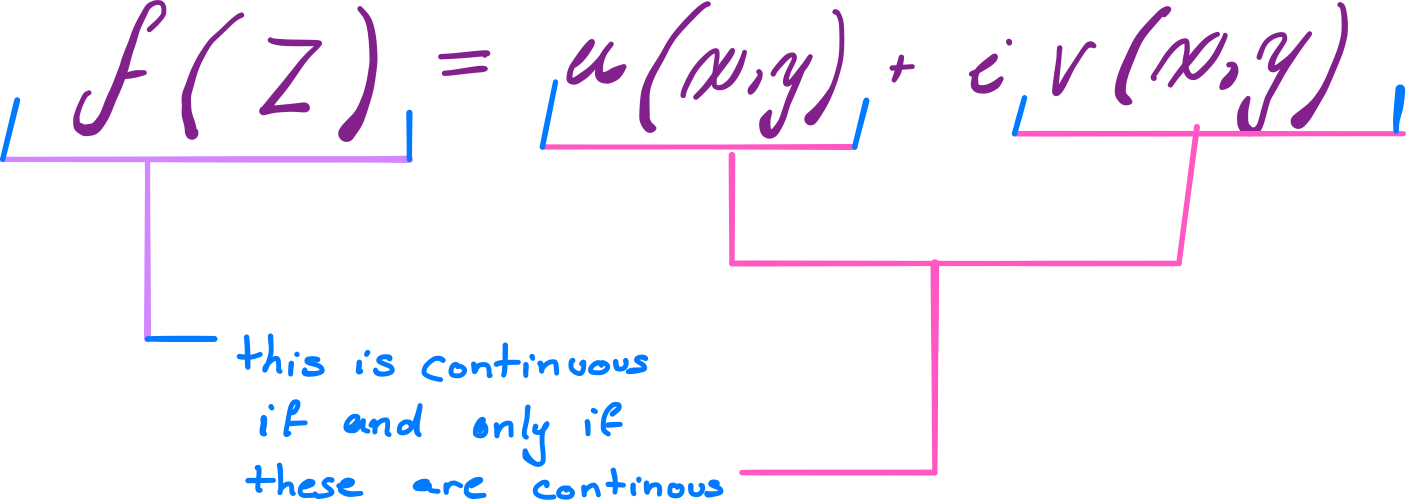
\includegraphics[width=0.7\linewidth]{"./media/ComplexFunctions/PNG image 4.png"}
%	\caption{}
	\label{fig:png-image-4}
\end{figure}

Again, remember this for later when we are doing the \textit{Cauchy Riemann} equations.


\newpage


\section{Derivatives}
Derivatives have the same definition in complex analysis as they do in real calculus, with the difference that the variable is now complex, the derivative of $f$ at $a$ is:

  \begin{align*}
    w &= f \left( z \right)\\
    &\implies \frac{\operatorname{d} w}{\operatorname{d} z} = \lim_{\Delta Z\rightarrow 0}\left[ \frac{\Delta w}{\Delta z} \right] 
  \end{align*}

Or in a more useful fashion:

\[
  f'\left( a \right) = \lim_{\Delta Z\rightarrow 0}\left[ \frac{f \left( z \right) - f \left( a \right) }{z - a} \right] = \lim_{\Delta Z\rightarrow 0}\left[ \frac{f \left( a + \Delta z \right) -  f \left( a \right) }{\Delta z} \right] 
\]

A function may be differentiable at a point $z$ but not necessarily at any other points in the neighbourhood of $z$. \\

The real and imaginary components of a function may have continuous partial derivatives (of all orders) yet this does not imply that the function is differentiable there, 

\ \

\hfill\begin{minipage}{\dimexpr\textwidth-3cm}
e.g.  $   f\left( z \right) =   \left| z \right|$ has continuous partial derivatives away from $z =  0$, but is not differentiable anywhere, because the limits as $\Delta   z  \rightarrow 0$ are different depending on which path is taken.\end{minipage}
\ \





\paragraph{Conditions of Continuity}
\begin{itemize}
  \item if a function is continuous it may or may not be differentiable
  \subitem continuity $ \centernot\implies $ differentiability
  \item if a function is differentiable it must be continuous
  \subitem differentiability $ \implies  $ continuity
\end{itemize}

\subsection{Derivatives to Memorise}
The following complex functions are nowhere differentiable:

\begin{itemize}
  \item $f\left( z \right)  = \Re{\left( z \right) }$ 
  \item $f\left( z \right) = \Im{\left( z \right) }  $ 
  \item $f\left( z \right)  = \overline{z}$ 
\end{itemize}

The function $f\left( z \right) =      \left| z \right|^{2}$ is differentiable only at $z =  0$:
\[
  \frac{\operatorname{d} }{\operatorname{d} z}\left(     \left| z \right|^{2} \right) \Big|_{z =  0} = f'\left( 0 \right) = 0
\]

bear in mind however that this function is nowhere analytic, because it is not differentiable on a neighbourhood of 0, this is covered further down.

\paragraph{How to Deal with Derivatives}
If you are given a function purely of $z$, then all the familiar differentiation rules carry over, their proofs are different, but the rules come out the same.  
\footnote{I mean, be careful with $\log$ functions and roots because they have multiple values}\\

If however you are given a function with terms of $z$, $x$ and $y$, then you will need to first break the function up into it's components:

\[
  f\left( z \right)  =  u\left( x,y \right) + i\cdot v\left( x,y \right) 
\]

and then you will need to use the \textit{Cauchy Riemann} equations, which we will get to further down.

\paragraph{Example}
Find the derivative of $w =  f\left( z \right) =  \frac{1}{z}$:

\end{document}
